\documentclass{article}
\usepackage[T1]{fontenc}
\usepackage{lmodern}
\usepackage{graphicx}
\usepackage{amsmath,amssymb}
\usepackage[a4paper,margin=2cm]{geometry}
\usepackage[absolute,overlay]{textpos}
\setlength{\TPHorizModule}{1mm}
\setlength{\TPVertModule}{1mm}
\usepackage[indonesian]{babel}
\usepackage{hyperref}
\setlength{\emergencystretch}{2em}
% unit: Halaman 8

\begin{document}

% === Halaman 8 (llm) ===

% (tidak ada teks dari model)

% deskripsi: Kumpulan delapan tabel (Kotak-S 1 sampai Kotak-S 8) yang berisi deretan angka acak dalam sel-sel tabel.
% bbox normalisasi: [0.1670, 0.0440, 0.8330, 0.9050]
\begin{textblock*}{139.86mm}(35.07mm,13.07mm)
\noindent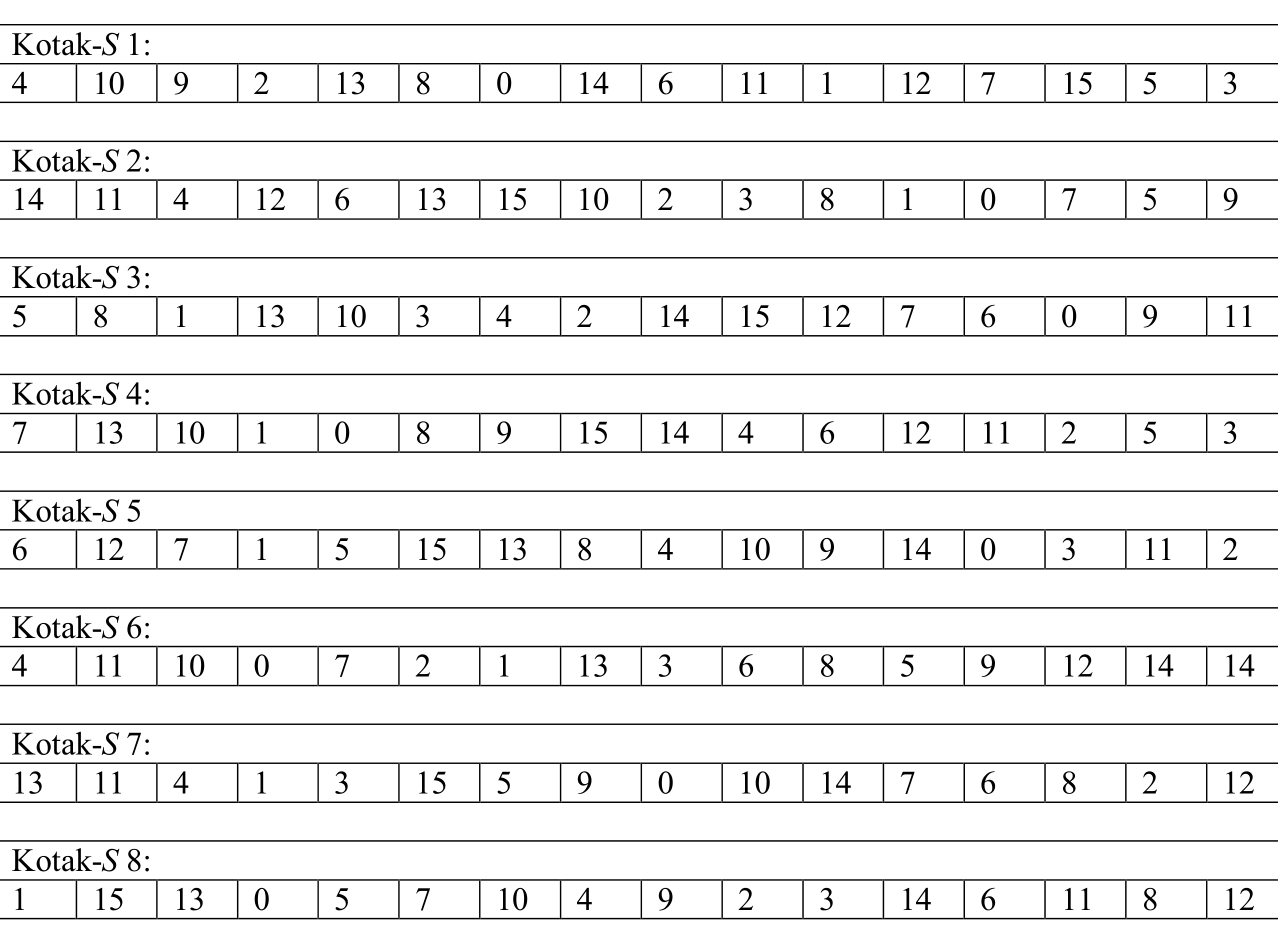
\includegraphics[width=139.86mm,height=255.72mm]{../../images/llm/page_008_img_01.png}%
\end{textblock*}

\end{document}
